\section{System Framework}

\subsection{Cloud Server Configuration}

\subsubsection{Memory and Cores}

The system architecture contains many components. The metastore of hive is deployed on mysql, so that hive can be used by multiple users. Therefore, we need to choose a server with large memory to accommodate all components. Considering the system requirements, we choose a server with 4 cores and 16G memory.


\subsubsection{Server Type}

Our task is to build a data analysis service platform that continuously obtains log information and do data analyze jobs. We chose preemptible instances because of their relatively low price. And we have developed a set of fully automated scripts to deploy the cluster, so that if the server needs to be released unexpectedly, the service can be easily deployed to the newly created server.


\begin{figure}[H]
    \centering
    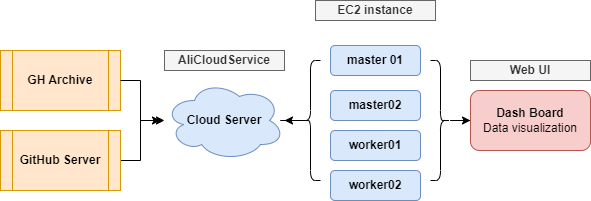
\includegraphics[width=0.45\textwidth]{./pic/server.png}
    \caption{A figure shows types of servers}
    \label{fig:server}
\end{figure}



\subsubsection{Final Cluster Choice}


For the final cluster, we use 4 server, which are named as \textit{master01}, \textit{master02}, \textit{worker01} and \textit{worker02}. Different server played as different character in the cluster.


The Server details information:
\begin{itemize}
    \item Instance type: Preemptible Instance
    \item Specifications: 4v CPU 16 GiB (I/O Optimized)
    \item Storage: 40GiB Cloud disk for each server
    \item Network: 100Mbps
\end{itemize}



\begin{figure}[H]
    \centering
    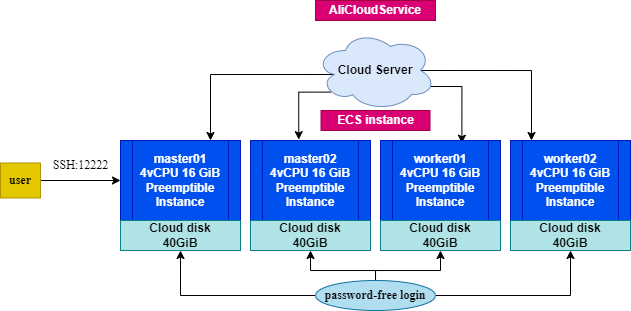
\includegraphics[width=0.45\textwidth]{./pic/server-info.png}
    \caption{A figure shows details configuration of clusters}
    \label{fig:server-info}
\end{figure}



\subsubsection{Auto Configuration}
Preemptive servers may be automatically released for lack of resources by Aliyun, so we need to purchase new computation instances, deploy the original big data system quickly and recover data collected when that worst situation happens. Based on this requirement, we have implemented a complete automatic configuration shell script, so that only one script need to be executed on any one single node to complete the environment configuration and deployment of the whole cluster, which greatly improves the efficiency of the cluster deployment and reduces the workload of the administrator.


\begin{figure}[H]
    \centering
    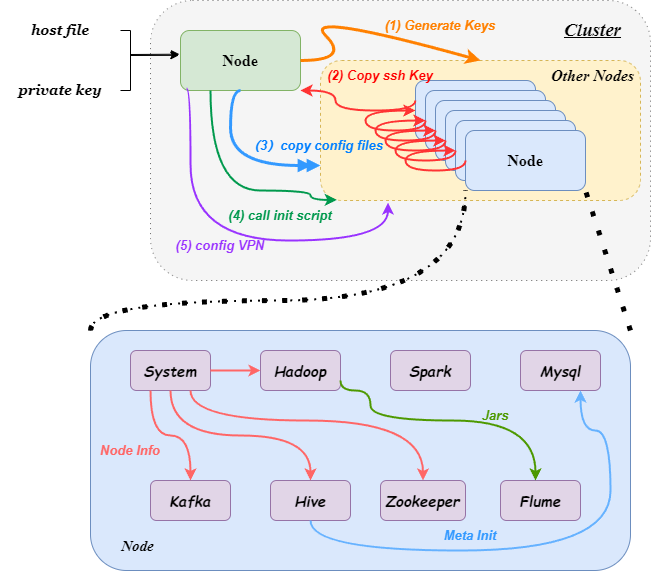
\includegraphics[width=0.5\textwidth]{./pic/autoconfig.png}
    \caption{A figure shows the control flow of auto configuration}
    \label{fig:autoconfig}
\end{figure}

\paragraph*{Cluster}
For the whole cluster:
\begin{enumerate}
    \item Upload private key (for log in server initially) and host file (record the ip and name of all nodes) to any one nodes \textit{A}.
    \item Execute autoconfig shell script, which will do the following things one by one:
    \begin{enumerate}
        \item Require each node to generate a new ssh key pair and update sshd configuration.
        \item Each node broadcasts its own public key to all other nodes for password-free login. Then only use the new own key to log in to other nodes after that.
        \item Synchronize all necessary config files of components(hadoop, spark, etc) from \textit{A} to all other nodes.
        \item Execture the installation script on each node's background.
        \item After the installation is complete, all nodes need to config a VPN proxy to access the outer Internet for downloading Github data.
    \end{enumerate}
\end{enumerate}

All big data components will be installed when installation script is executed. The installation script will do the following things one by one on each node:
\begin{enumerate}
    \item Install system software, update system environment variables and create necessary directories.
    \item Modify configuration files of each component according to the node's role and special information, such as zookeepers'id, etc.
    \item Download and install all components one by one, and copy the configuration files to the corresponding location.
    \item Copy essential \textbf{\textit{Jars}} of hadoop and spark to other components' \textit{lib} directory, such as flume, which is used for ensure consistence of the version of all components to avoid potential problems.
    \item MySQL will be installed on \textit{worker02}, modify access authority, and init database schema. The JDBC driver will be installed on all nodes.
    \item Init hive metastore database on \textit{worker02}. The hive schema will be stored in MySQL.
\end{enumerate}



\subsubsection{Security Control}    
After deployment, servers are frequently attacked from unknown sources, including DDoS, mining viruses, worms, and remote controlling, which causes the extremely high CPU usage, high disk IO, and unable to access the server. Killing processes, resetting servers, and recollecting data took up over 40\% of our time.


Although it has been observed that the behavior after entering the server is to inject code into the process, it is not clear by what means the server was successfully accessed and permissions obtained. We have taken the following steps to try to avoid being attacked:

\begin{itemize}
    \item \textbf{Change the default port of sshd}: The default port of sshd is 22, which is the most frequently attacked port. We changed the port to 2222, which greatly reduced the number of attacks.
    \item \textbf{Only allow strict key login}: Some instruction of automated configuration steps need to be provided password, we generated a random length of 40 characters password by openssl and only use it once. After the configuration is complete, the password will be deleted, and all communication will be based on the rsa key.
    \item \textbf{Close unnecessary ports}: We only preserve port for ssh login and data visualization for external network access, and other ports of big data components are only open to the internal network.
    \item \textbf{Install anti-virus software}: We installed \textit{ClamAV} on each node to scan the system periodically.
\end{itemize}

All above measures cannot completely prevent attacks, and we believe there is an unknown vulnerability in linux system or big date components. The corresponding logs are in the Appendix \ref{a-sec}.




\subsection{System Architecture}
Our goal is to build a distributed file system and computing analysis system based on cloud servers. After identifying the servers and clusters, we need to decide where to deploy the components and how data will flow between the different components within the architecture.



\subsubsection{Technology selection}

Considering our needs, we need to build a distributed file system and distributed computing system for continuously input log information, and need to store related information such as users and warehouses. So we choose the most commonly used technology in the field of big data: Hadoop architecture. Considering the data form we need, we use hive to store the data as hive tables. For faster analysis, we use spark for distributed computing and analysis. According to the main thread, we add more components to it to maintain the continuous operation of the whole system.



\subsubsection{Deployment}

\begin{figure}[H]
    \centering
    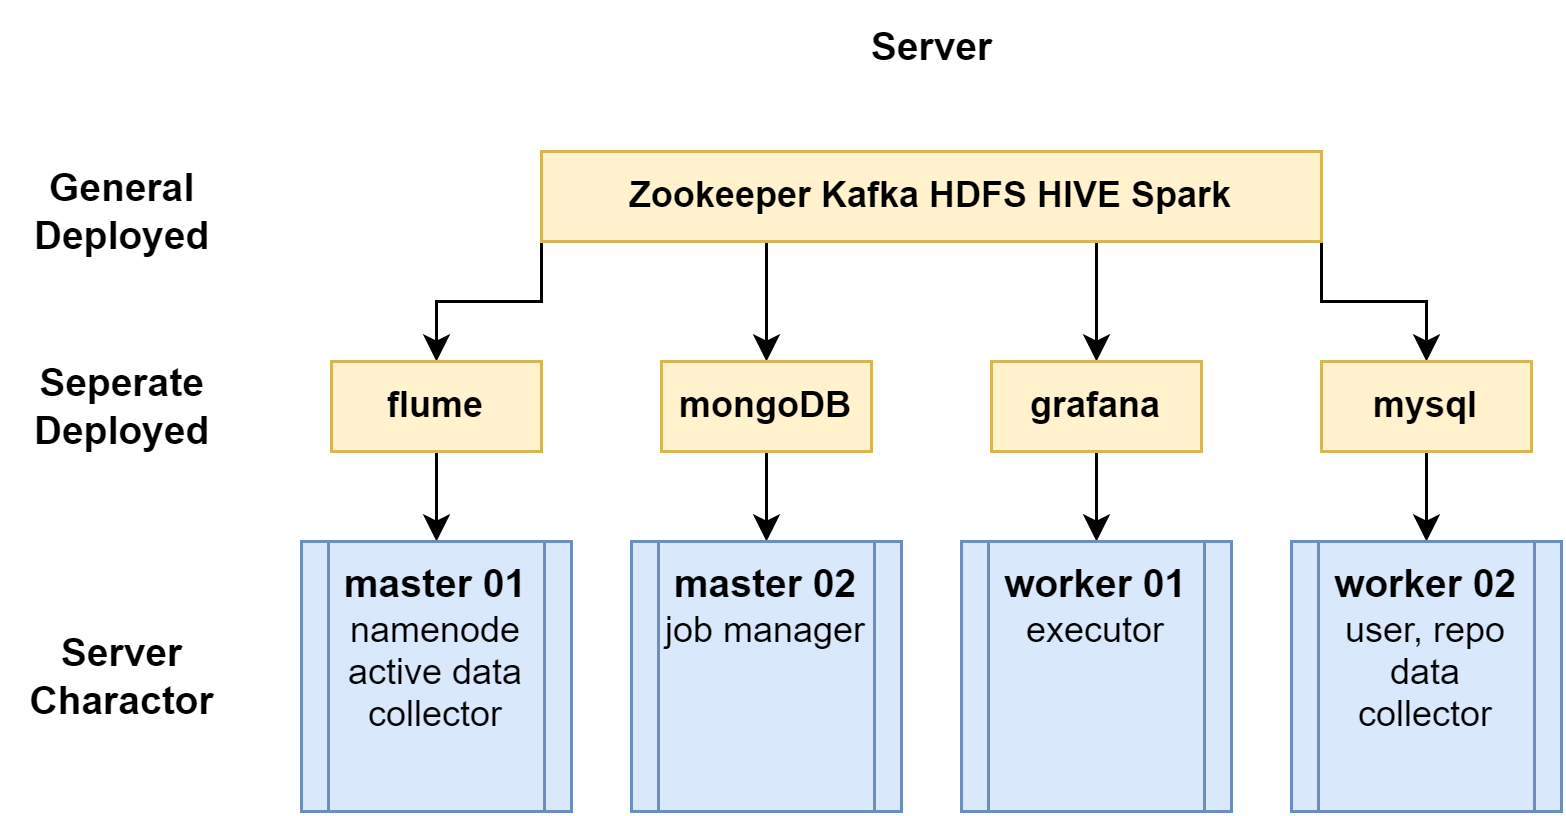
\includegraphics[width=0.5\textwidth]{./pic/deploy.png}
    \caption{A figure show the deployment of the system}
    \label{fig:deploy}
\end{figure}

Balance the server workload so that the cluster can perform at its best. Therefore, it is important to plan the placement of components. Below are the locations of the different components on the server and their basic functionality.


For the entire analysis system we use the following components. Here we briefly introduce these components:

\begin{enumerate}
    \item \textbf{Zookeeper}: ZooKeeper is a centralized service for maintaining configuration information, naming, providing distributed synchronization, and providing group services.[1] https://zookeeper.apache.org/
    \item \textbf{Kafka}: message queue, which temporarily stores data and sends it downstream. It is the data source and key part of subsequent data stream processing.
    \item \textbf{Hadoop}: Hadoop includes HDFS, Yarn and MapReduce. HDFS is the main storage place where we store data. HDFS is deployed on each server. Use Yarn as a resource manager. The resource manager is deployed on master02.
    \item \textbf{Hive}: Hive data is stored in HDFS. The hive engine is very inefficient, so only use hive as storage and data management on HDFS. Hive is deployed on the entire cluster.
    \item \textbf{Spark}: Spark is deployed on the entire cluster as the main component for data processing and data analysis. Also use \textbf{Spark Streaming} to process real-time data streams.
    \item \textbf{MySQL}: The data of users and warehouses are stored in MySQL, and MySQL is deployed on worker02. At the same time, the hive meta store is also on MySQL.
    \item \textbf{Flume}: Track the data in the data capture folder and transfer it to Kafka. It will also transfer data from Kafka into a temporary folder in HDFS. The data capture process is deployed on worker02.
    \item \textbf{MongoDB}: MongoDB is deployed on master02 for expose the API. The data is stored in json format, which facilitates a background application such as flask to respond to web requests. We have stored analysis results in MongoDB.
    \item \textbf{Grafana}: Grafana is deployed on worker01. It's the interface of data visualization. It can connect to MySQL to get data and display it in the form of charts. In fact, it get well-structure data by constructing SQL statements and then send it to MySQL for processing. It's easy to combine single figure into a  dashboard. Grafana also provides port mapping for external network access.
\end{enumerate}


The version of key components will be listed in the Appendeix\ref{a-version}.



\subsection{Data Flow}

\begin{figure}[H]
    \centering
    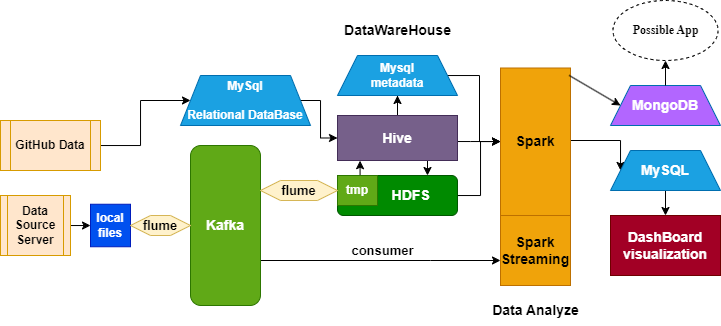
\includegraphics[width=0.4\textwidth]{./pic/dataflow.png}
    \caption{A figure shows the data flow of the system}
    \label{fig:dataflow}
\end{figure}


The server structure section introduces the general data flow direction, and here is a detailed description of the data flow in the overall analysis system.

\paragraph*{1. Data source}
The data sources are divided into two parts.
The first part is GitHub user behavior log information. The source of this part of the information is the GitHub Archive website, from which one hour of data can be obtained every hour. We temporarily store the acquired data in a folder of worker02 through the Python program for subsequent data capture.
The second part is GitHub user personal information and repo information. The source of this part of information is the official server API provided by GitHub. We use Python crawlers to obtain user and repo data through these APIs and write them into the MySQL database, and the database keeps updating these data.

\paragraph*{2. Data transmission channel}
Data transmission channels mainly include flume and kafka.
The obtained log information tracks the file information through Flume, and transmits the continuously arriving data content to Kafka. Kafka internal data can be used by spark streaming through consumer. At the same time, Kafka and HDFS are connected through flume. The data accumulated in Kafka is consumed in batches and stored in the temporary folder of HDFS.

\paragraph*{3. Data load}
MySQL memory has continuously updated user and repository information. The temporary folder of HDFS has continuously added log information. We incrementally synchronize MySQL data to Hive through the spark program. Build it into a Hive table. The data of the Hive table is stored in HDFS.
At the same time, the log information in the temporary folder is imported through Hive, and the original data is transferred to Hive for subsequent use by using the JSON serde parsing package.

\paragraph*{4. Data Warehouse Construction}
Build a data warehouse based on the acquired data. The details will be explained later.

\paragraph*{5. Data analysis}
Spark directly extracts the data in the Hive data warehouse to analyze various indicators through the built data warehouse, and writes the analyzed results into multiple different databases for different purposes:
Write to MySQL for subsequent data display.
Write to MongoDB to expose Api externally.
Write to Hive for historical data storage.
Spark streaming directly obtains data through kafka for real-time data processing, so as to obtain updated and fast real-time data display.




\subsection{Data Warehouse Construction}



\subsubsection{Modeling}


\begin{figure}[H]
    \centering
    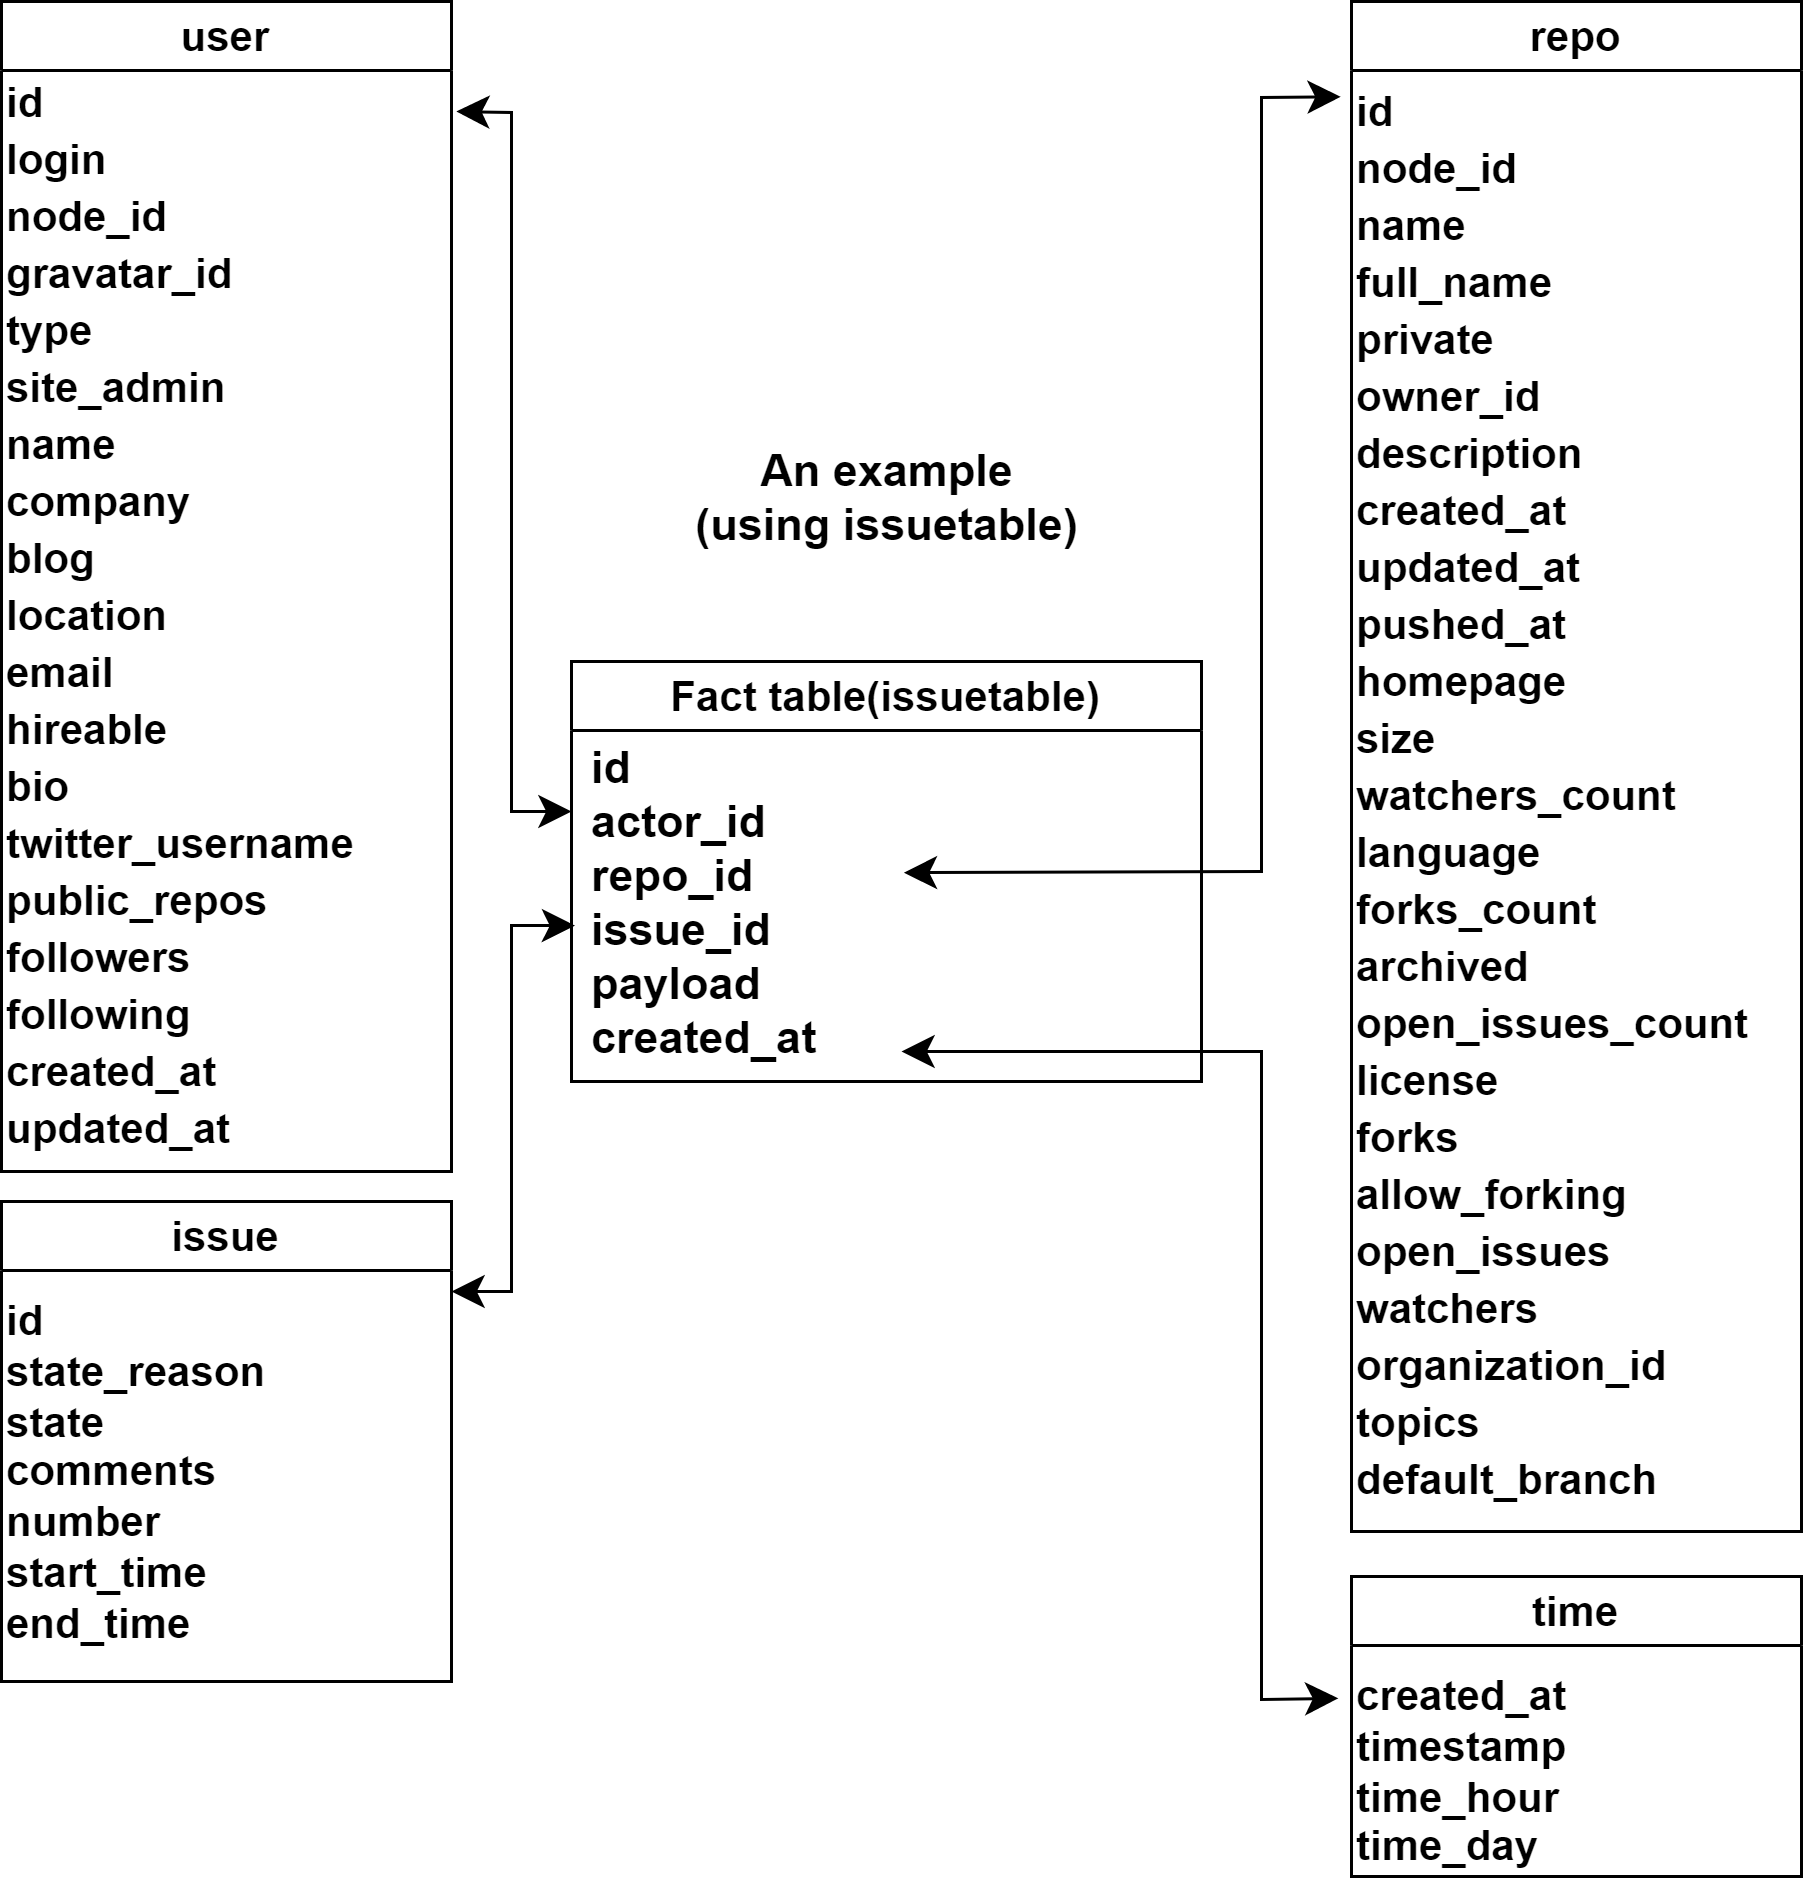
\includegraphics[width=0.45\textwidth]{./pic/tables.png}
    \caption{A figure shows the schema of the data warehouse}
    \label{fig:tables}
\end{figure}



The basic structure of data warehouse modeling adopts constellation model. There is a star schema for each transaction table, and different transaction tables share the same dimension table to form the entire constellation model.

Data granularity selection: The log data itself comes from every operation of GitHub users, and there is a corresponding time record for each operation. Since the data is acquired in one batch at the same time during the data acquisition process, the time granularity is selected to be as fine as 1 hour.

Determination of dimension table and transaction table: the dimension table adopts four dimensions of user, repo, issue and time, and the transaction table is divided into 8 types of transaction tables, such as create, delete, pull, and push, according to the different behavior of users.




\subsubsection{Hierarchy}


\begin{figure}[H]
    \centering
    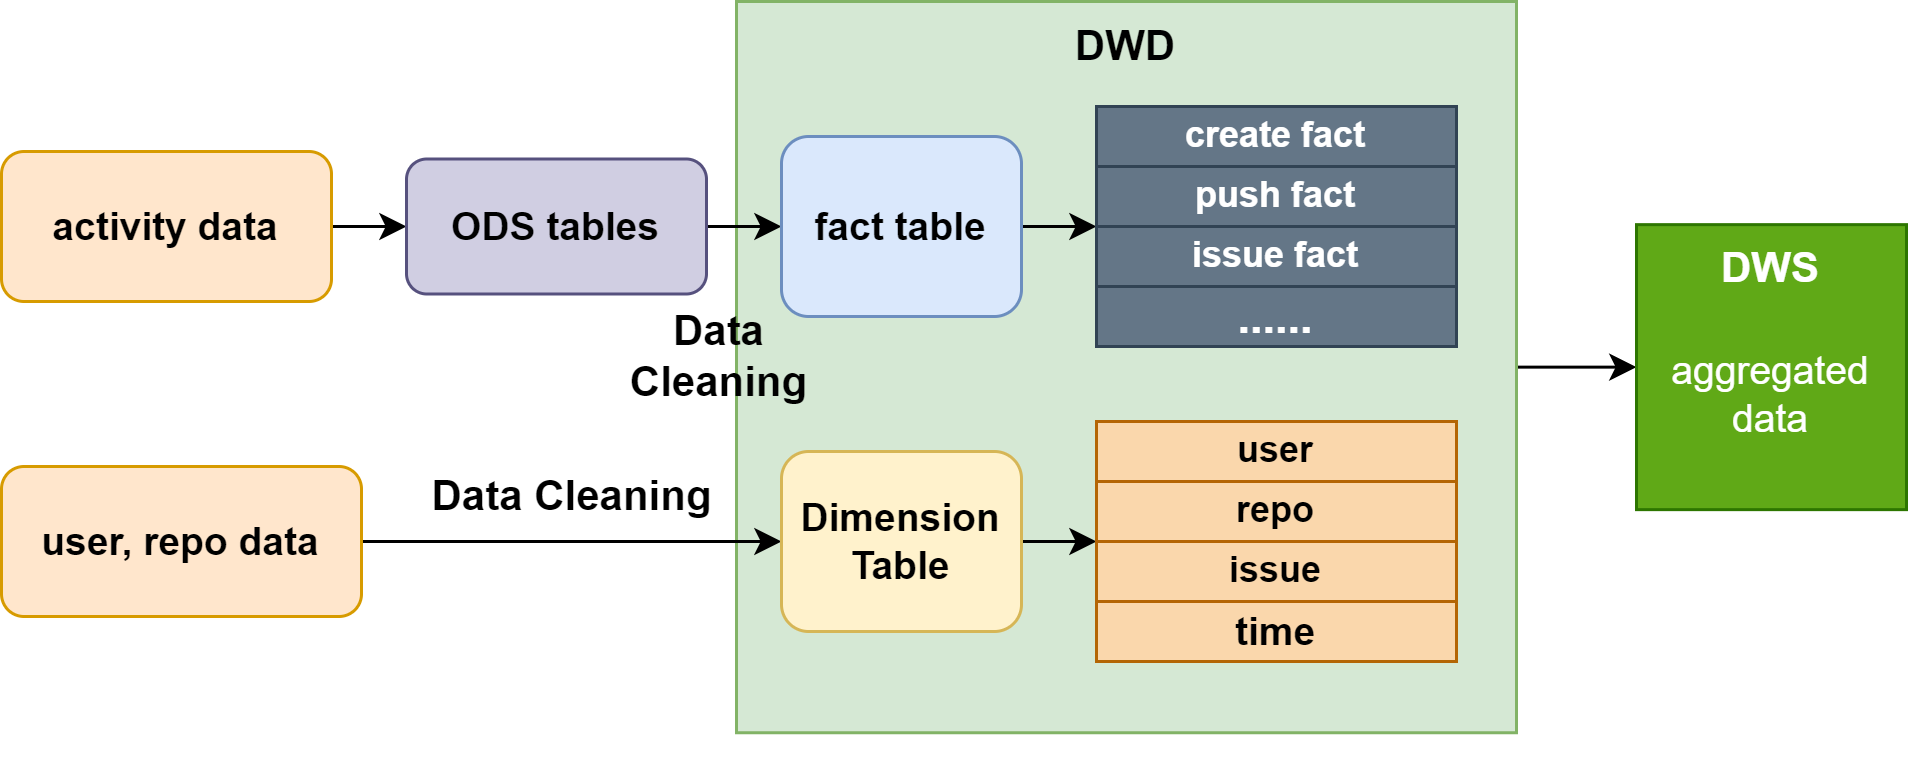
\includegraphics[width=0.5\textwidth]{./pic/warehouse.png}
    \caption{A figure shows details of the data warehouse}
    \label{fig:}
\end{figure}

\begin{itemize}
    \item \textbf{ODS layer}: When data is imported into Hive through the HDFS temporary data storage folder, the initial ODS layer table is formed. The ODS table stores the initial data without any data cleaning and processing.
    \item \textbf{DWD layer}: The data of the DWD layer comes from ODS and MySQL. The first is the transaction table. The data in the ODS layer is cleaned and preprocessed through the Spark program, invalid data and useless attributes are removed, valid information is screened, the retained content is determined, and the data is sorted out. Finally, different styles of data tables are constructed according to the type of data. These tables are all derived from the original user activity data of the ODS layer and the transaction tables are finally constructed. Then there are dimension tables. The specific information of the dimension table has already been determined, and there is synchronously updated data in MySQL. For the synchronization update process of MySQL, incremental synchronization will be performed in Hive to import data. Therefore, historical information of users and repo data will also be stored in Hive.
    \item \textbf{DWS layer}: Aggregate data at different levels for existing historical data information. After data aggregation for different time spans, the snapshot information is saved in the Hive data table to form various basic indicator results.
    \item \textbf{Data display}: Spark will use these basic indicators for analysis and processing, and transfer the results to the MySQL database for data display.
\end{itemize}





